% CVPR 2026 Paper Template; see https://github.com/cvpr-org/author-kit

\documentclass[10pt,twocolumn,letterpaper]{article}

%%%%%%%%% PAPER TYPE - PLEASE UPDATE FOR FINAL VERSION
% \usepackage{cvpr}              % To produce the CAMERA-READY version
% \usepackage[review]{cvpr}      % To produce the REVIEW version
\usepackage[pagenumbers]{cvpr} % To force page numbers, e.g. for an arXiv version

% Import additional packages in the preamble file, before hyperref
\input{preamble}

\definecolor{cvprblue}{rgb}{0.21,0.49,0.74}
\usepackage[pagebackref,breaklinks,colorlinks,allcolors=cvprblue]{hyperref}
\usepackage{multirow}
\usepackage{xcolor}

%%%%%%%%% PAPER ID - PLEASE UPDATE
\def\paperID{*****}
\def\confName{CVPR}
\def\confYear{2026}

%%%%%%%%% TITLE - PLEASE UPDATE
\title{Comprehensive Road Scene Understanding\\
for Autonomous Driving}

%%%%%%%%% AUTHORS - PLEASE UPDATE
\author{Xiangxi Li\\
s336719
\and
Kutay Zilcioglu\\
s364115
\and
Fabio Segalin\\
s363331
\and
Xueyufei Zhang\\
s336472
}

\begin{document}
\maketitle


\begin{abstract}
Safe autonomous driving requires efficient anomaly detection and semantic segmentation. In our work, we investigate the potential of the \textcolor{blue}{Encoder-only Mask Transformer (EoMT)} framework in relation to its cross-domain and fine-tuning properties. Specifically, we evaluate the transferability of an EoMT pre-trained on the \textcolor{blue}{Common Objects in Context (COCO)} panoptic segmentation task on the Cityscapes validation set. To overcome possible domain discrepancy, we propose two fine-tuning strategies, namely head-only and last-block fine-tuning. Moreover, we investigate how well EoMT models can perform out-of-distribution (OOD) anomaly detection using multiple post-hoc uncertainty estimates based on maximum logit, max entropy, and \textcolor{blue}{Rejected by All (RbA)}. In comparison with a generic pixel-based architecture like \textcolor{blue}{Efficient Residual Factorized ConvNet (ERFNet)}, we show that the usage of the EoMT framework along with the max entropy score is extremely encouraging to detect dangerous anomalies. Our code is available: \url{https://github.com/PoliTO-FAIMDL2526-Group51/image_segmentation}.
\end{abstract}



\section{Introduction}

Autonomous driving needs reliable road-scene understanding, and segmentation is one of the main tools for this because it assigns labels to image regions at pixel level. At the beginning of the project, we reviewed several segmentation tasks and models. ERFNet~\cite{romera2017erfnet} was used as an example of an efficient semantic segmentation model for real-time applications, while Panoptic Segmentation~\cite{kirillov2019panoptic} introduced the idea of combining semantic labels with instance-level information. We then studied mask-based methods, starting from MaskFormer~\cite{cheng2021per} and Mask2Former~\cite{cheng2022masked}, which treat segmentation more as a mask classification problem. \mbox{DINOv2}~\cite{oquab2023dinov2} and EoMT~\cite{kerssies2025your} were also relevant because they show how strong \textcolor{blue}{Vision Transformer (ViT)} features can be used for segmentation. Based on this background, Step 4 compares two pretrained EoMT models: one trained on Cityscapes for semantic segmentation and one trained on COCO for panoptic segmentation. Since their tasks and label spaces are different, we mapped their predictions to a common semantic label space and evaluated them on the Cityscapes validation set using \textcolor{blue}{mean Intersection over Union (mIoU)}. In step 5 we have analyzed how well the COCO EoMT model can perform when fine-tuned with Cityscapes. We used two different lightweight approaches, head-only and last-block fine-tuning.
Before evaluating the mask-based architecture, we ran the dataset through the traditional network to measure the pixel baselines, and compare the improvement in performance.
Finally, we evaluate the mask-based EoMT checkpoints for anomaly segmentation in open-world road scenes. We apply \textcolor{blue}{Maximum Softmax Probability (MSP)}, MaxLogit, MaxEntropy, and the mask-specific RbA~\cite{nayal2023rba} to detect pixels outside the known road-scene distribution. We also study how checkpoint training and temperature scaling affect anomaly detection across five benchmark datasets.


\section{Methodology}


As required in step 4, we compare the two provided EoMT checkpoints on the Cityscapes validation set. The two models are:

\begin{itemize}
    \item \texttt{eomt\_cityscapes.bin}, trained on Cityscapes for semantic segmentation.
    \item \texttt{eomt\_coco.bin}, trained on COCO for panoptic segmentation.
\end{itemize}

We use the \texttt{eomt} code from the provided course repository, instead of rewriting the model architecture. In particular, the EoMT model definition, the ViT backbone, the semantic segmentation module, the panoptic segmentation module, and the corresponding config files are loaded from the repository.

The Cityscapes validation set is loaded from the official zip files:

\begin{itemize}
    \item \texttt{leftImg8bit\_trainvaltest.zip}
    \item \texttt{gtFine\_trainvaltest.zip}
\end{itemize}


Since the two models are trained on different datasets and tasks, their output classes are not directly comparable. To make the comparison more consistent, both outputs are mapped into a smaller common label space. The common classes used are:

\begin{center}
\texttt{road, sidewalk, building, wall, fence, vegetation, sky, person, car, bus, truck, bicycle, motorcycle, train, traffic light}
\end{center}

For the Cityscapes model, the output is already a semantic segmentation prediction, so the Cityscapes train IDs are mapped to the common classes. For the COCO model, the panoptic output is first converted into semantic class labels, and then the COCO labels are mapped into the same common class space.

The final metric is mean Intersection over Union (mIoU), computed on the full Cityscapes validation set. \cref{fig:step4_comparison} is an example.

\begin{figure}[h]
    \centering
    % Replace the path below with the selected visualization image.
    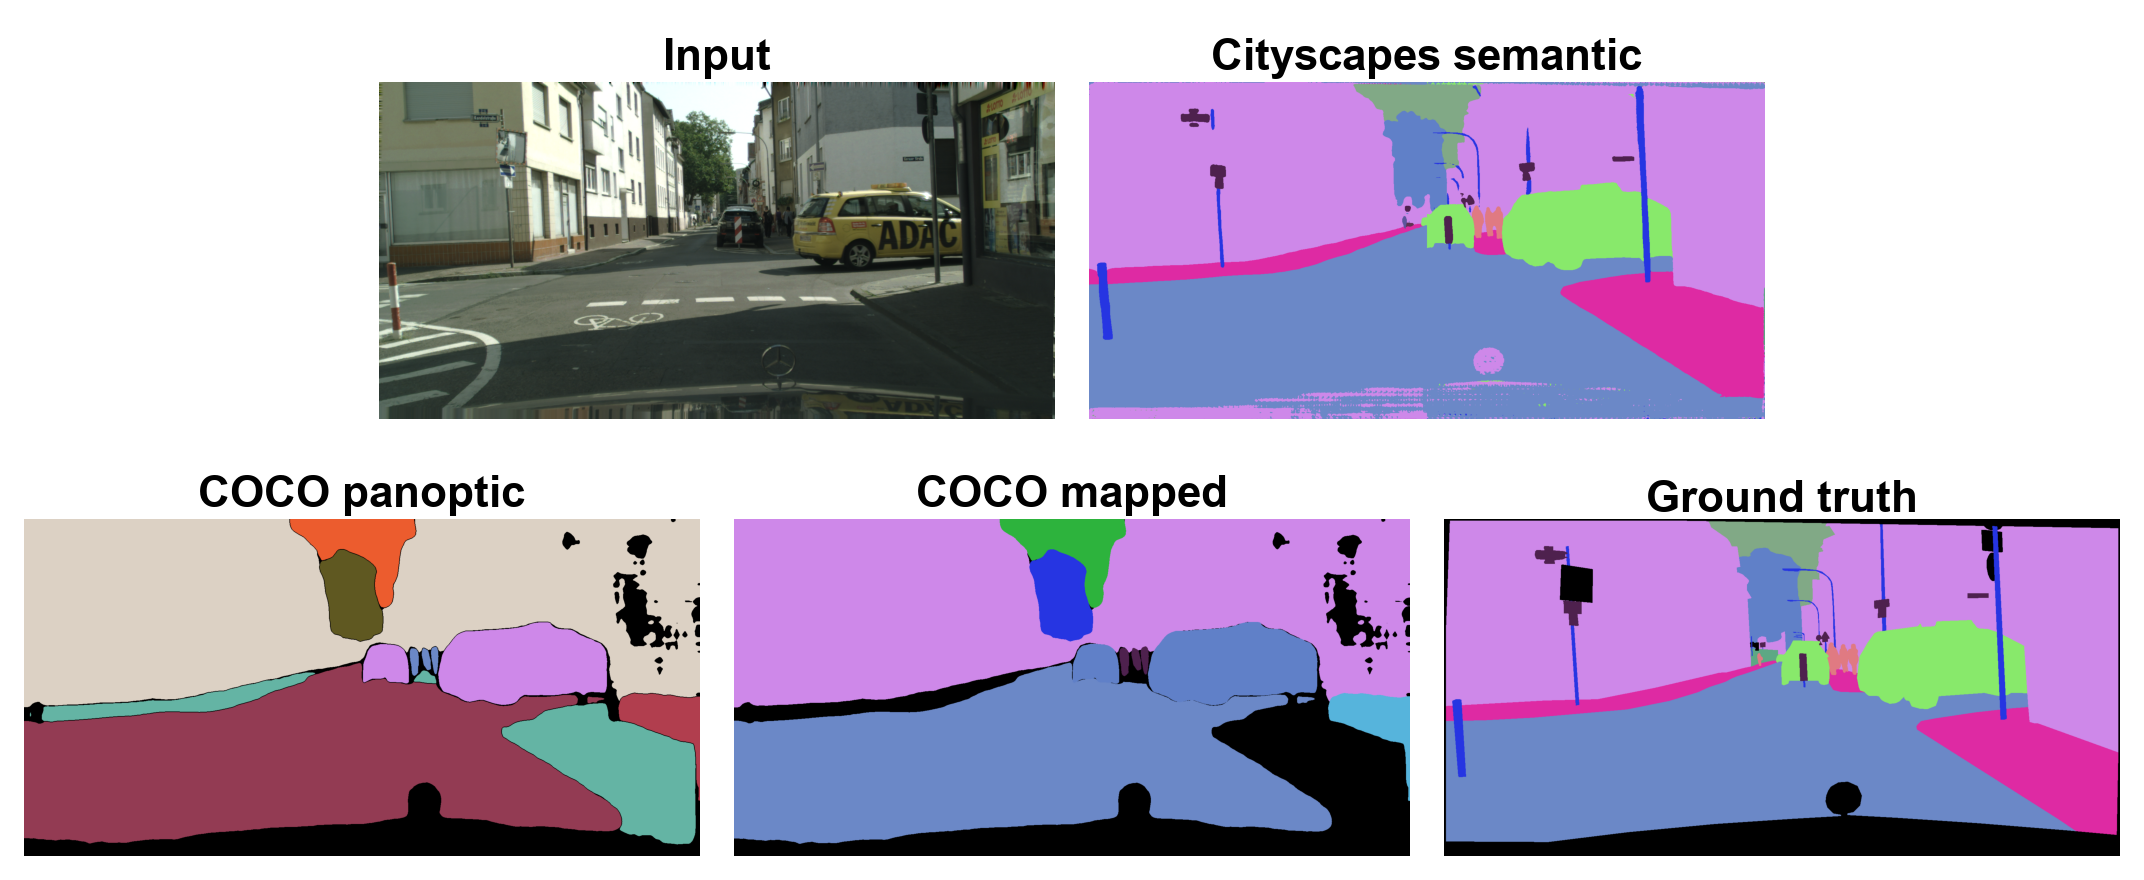
\includegraphics[width=0.5\textwidth]{example.png}
    \caption{Comparison between the two EoMT models. The visualization shows the input image, the Cityscapes EoMT semantic prediction, the COCO EoMT panoptic prediction, the COCO prediction mapped to the common label space, and the Cityscapes ground truth.}
    \label{fig:step4_comparison}
\end{figure}

To understand how well COCO EoMT can be adapted to Cityscapes, we performed a fine-tuning approach as indicated in step 5. 

In the first experiment, we only trained parameters belong to the head. We chose this approach to make the experiment more affordable and complicated enough to examine significant changes. Specifically, the trained parts are query embeddings, class head, mask head, upscale layers. 

In our second experiment to evaluate a more widespread fine-tuning approach was used by unfreezing the last ViT block and final normalization layer. This allows the model to adapt part of the backbone representation to the Cityscapes domain, while still keeping most of the pretrained encoder frozen. The purpose of this experiment is to evaluate whether limited backbone adaptation improves over head-only fine-tuning.

Before evaluating the mask-based architecture, the pixel-based baselines were calculated using ERFNet, a conventional CNN. Its results would be compared to the performance of EoMT, establishing whether it handles anomalies better than traditional pixel classifiers.

To detect anomalies, three post-hoc methods were used, as ERFNet is just a semantic segmentation model, not an anomaly detector, and thus detection is done from the segmentation outputs

\begin{itemize}
    \item \texttt{Maximum Softmax Probability}, computed as 1 - maximum class probability.
    \item \texttt{MaxLogit}, looking at the negative of the maximum raw logit.
    \item \texttt{MaxEntropy}, taking into account the high entropy score of the softmax distribution.
\end{itemize}

Two performance metrics were used for each method across the different datasets, keeping the same preprocessing and evaluation pipeline:  \textcolor{blue}{area under the Precision-Recall Curve (AuPRC)}, and  \textcolor{blue}{false positive rate at 95\% true positive rate (FPR95)}.

\paragraph{Mask-Based Anomaly}EoMT predicts $Q$ query masks $M_q$ and query-level class logits $\mathbf{z}_q$.
They are aggregated into the per-pixel semantic score
\begin{equation}
S_c(i)=\sum_{q=1}^{Q}
    \text{softmax}(\mathbf{z}_q)_c\,\sigma(M_q(i)),
\label{eq:aggregation}
\end{equation}
excluding the no-object class. From $\mathbf{p}(i)=\text{softmax}(\mathbf{S}(i))$, we
compute MSP, MaxLogit, and normalized MaxEntropy using the same definitions as the
pixel baseline. The mask-specific score is
\begin{equation}
    A_{\mathrm{RbA}}(i)=-\sum_c\tanh(S_c(i)).
\label{eq:rba}
\end{equation}
Temperature scaling replaces
$\text{softmax}(\mathbf{z}_q)$ in \cref{eq:aggregation} with
$\text{softmax}(\mathbf{z}_q/T)$ for
$T\in\{0.25,0.5,0.75,1,1.5,2,2.5\}$.

We evaluate EoMT trained on COCO and Cityscapes, plus the Step 5 head-only and
last-block fine-tuned checkpoints. All four scores are evaluated on \textcolor{blue}{\mbox{SegmentMeIfYouCan} (SMIYC), RoadAnomaly21 (RA-21), RoadObstacle21 (RO-21), FishyScapes (FS) Lost \& Found, FS Static, and Road Anomaly}.
Results use AuPRC (higher is better) and FPR95 (lower is better).

\section{Experimental Results}

\subsection{Main Results}

In step4, The main result is reported on the full Cityscapes validation set. The Cityscapes-trained EoMT checkpoint, \texttt{eomt\_cityscapes.bin}, achieved an mIoU of 0.8582. In comparison, the COCO-trained EoMT checkpoint, \texttt{eomt\_coco.bin}, achieved an mIoU of 0.6198 after its panoptic predictions were mapped to the common semantic label space.

The Cityscapes-trained model performs better, which is expected because it was trained on the same dataset style and on the same type of task used for evaluation. The COCO-trained model still gives meaningful predictions, but its score is lower because it was originally trained for panoptic segmentation on a different dataset and label space.

Fine-tuning approaches give some noticeable increase of mIoU metric which can be observed in \cref{tab:main-results}. For head-only tuning the mIoU value reached 0.8 while last-block method scores a mIoU value of 0.81. Adapting the COCO-trained model to the Cityscapes dataset improves its segmentation performance.
\begin{table*}[t]
\centering
\caption{Post-hoc pixel-based baselines on ERFNet. Cells: AuPRC$\uparrow$ /
  FPR95$\downarrow$ (\%).}
\label{tab:pixel-based baselines}
\setlength{\tabcolsep}{3pt}
\scriptsize
\resizebox{\textwidth}{!}{%
\begin{tabular}{ll cccccc}
\toprule
Model & Method & Road Anomaly & SMIYC RA-21 & SMIYC RO-21 & FS Static & FS L\&F \\
\midrule
\multirow{4}{*}[0.5em]{ERFNet}
    & MSP & \textbf{12.43/82.59} & \textbf{29.09/62.62} & \textbf{2.71/65.22} & \textbf{7.43/41.84} & \textbf{1.75/50.60} \\
    & MaxLogit & 15.55/73.31 & 38.30/59.41 & 4.63/48.44 & 9.44/40.30 & 3.30/45.50 \\
    & MaxEntropy & 12.67/82.74 & 30.96/62.74 & 3.04/65.91 & 8.78/41.58 & 2.58/50.16 \\
\bottomrule
\end{tabular}}
\end{table*}

\begin{table*}[h]
\centering
\caption{Post-hoc anomaly segmentation on EoMT ($T{=}1$). Cells: AuPRC$\uparrow$ /
  FPR95$\downarrow$ (\%).}
\label{tab:main-results}
\setlength{\tabcolsep}{3pt}
\scriptsize
\resizebox{\textwidth}{!}{%
\begin{tabular}{ll cccccc}
\toprule
Model & Method & mIoU & Road Anomaly & SMIYC RA-21 & SMIYC RO-21 & FS Static & FS L\&F \\
\midrule
\multirow{4}{*}{EoMT Cityscapes}
    & MSP & 0.85 & 71.3/15.4 & 68.4/30.0 & 93.4/0.5 & 22.9/40.0 & 16.3/13.0 \\
    & MaxLogit && 70.7/15.1 & 67.7/31.3 & 93.5/0.5 & 22.9/46.6 & 16.3/12.9 \\
    & MaxEntropy && \textbf{73.3/14.6} & 68.5/30.4 & 93.6/0.5 & 26.5/40.0 & 18.7/12.8 \\
    & RbA && 70.1/15.2 & 62.7/96.3 & 93.2/0.5 & 24.2/78.5 & 16.4/\textbf{9.1} \\
\midrule
\multirow{4}{*}{EoMT COCO}
    & MSP & 0.61 & 18.1/98.7 & 24.2/77.9 & 1.3/100.0 & 2.2/96.7 & 1.5/97.2 \\
    & MaxLogit && 18.2/98.7 & 24.8/77.3 & 1.3/100.0 & 2.2/96.6 & 1.5/97.2 \\
    & MaxEntropy && 19.5/98.6 & 33.2/51.1 & 2.1/100.0 & 2.1/95.8 & 1.4/96.9 \\
    & RbA && 15.1/78.2 & 22.4/59.7 & 9.5/100.0 & 1.0/94.3 & 0.2/97.7 \\
\midrule
\multirow{4}{*}{EoMT FT-Head}
    & MSP & 0.8 & 59.5/32.9 & 73.4/28.8 & 73.5/1.0 & 79.1/8.1 & 43.7/15.2 \\
    & MaxLogit && 58.6/33.0 & 72.9/31.9 & 72.5/1.0 & 78.8/7.9 & 43.3/19.1 \\
    & MaxEntropy && 58.6/33.1 & \textbf{73.4/27.7} & 71.6/0.9 & 79.0/7.0 & \textbf{43.9}/20.6 \\
    & RbA && 51.0/83.8 & 56.5/96.9 & 54.5/93.0 & 69.9/79.0 & 37.5/89.8 \\
\midrule
\multirow{4}{*}{EoMT FT-LastBlock}
    & MSP & 0.81 & 62.1/24.9  & 67.1/40.0 & 94.2/0.3 & 86.0/4.7 & 35.3/19.1 \\
    & MaxLogit && 61.5/24.3  & 64.7/81.2 & 94.2/0.3 & 86.0/4.5 & 35.6/17.9 \\
    & MaxEntropy && 63.1/23.8  & 65.2/81.4 & \textbf{94.5/0.3} & \textbf{86.3}/3.9 & 37.2/17.4 \\
    & RbA && 58.9/19.0  & 49.1/98.4 & 92.2/0.4 & 84.4/\textbf{3.8} & 36.5/78.6 \\
\bottomrule
\end{tabular}}
\end{table*}

The raw COCO checkpoint is consistently the weakest anomaly detector because its broad known-class vocabulary includes many objects considered anomalous in road scenes. Adapting the model to Cityscapes greatly improves anomaly detection, but there is no universally best fine-tuning depth: \textcolor{blue}{the head-only fine-tuned model (FT-Head)}, \textcolor{blue}{the last-block fine-tuned model (FT-LastBlock)}, and the Cityscapes checkpoint each perform best on different datasets. Among the post-hoc scores, MaxEntropy is the most reliable default, whereas RbA is substantially less stable across datasets and operating points. Temperature scaling can improve ranking, but its effect depends on the checkpoint, dataset, score, and target metric.

\subsection{Quantitative Breakdown}

\begin{table}[t]
    \centering
    \caption{Per-class IoU comparison after mapping both models to the common evaluation label space.}
    \label{tab:step4_per_class}
    \begin{tabular}{lcc}
        \hline
        Class & Cityscapes EoMT & COCO EoMT \\
        \hline
        road & 0.9852 & 0.9791 \\
        sidewalk & 0.8925 & 0.0000 \\
        building & 0.9523 & 0.9015 \\
        wall & 0.6718 & 0.5338 \\
        fence & 0.6783 & 0.5406 \\
        vegetation & 0.9483 & 0.9068 \\
        sky & 0.9583 & 0.8989 \\
        person & 0.8781 & 0.7886 \\
        car & 0.9592 & 0.8437 \\
        bus & 0.9072 & 0.7291 \\
        truck & 0.8223 & 0.2908 \\
        bicycle & 0.8542 & 0.7235 \\
        motorcycle & 0.7814 & 0.6886 \\
        train & 0.7813 & 0.0000 \\
        traffic light & 0.8026 & 0.4726 \\
        \hline
    \end{tabular}
\end{table}

From the \cref{tab:step4_per_class}, the Cityscapes model is more stable across almost all classes. The COCO model still gives good results for some common categories, such as road, building, vegetation, sky, person, and car. However, it fails or performs poorly for some classes where the mapping between COCO and Cityscapes is weak, such as sidewalk and train.

At $T=1$, MaxEntropy with FT-Head obtains the highest AuPRC on RA-21 and Lost \& Found; FT-LastBlock is highest on RO-21 and FS Static; and Cityscapes is highest on Road Anomaly. FT-LastBlock has the highest mean MaxEntropy AuPRC across the five datasets (69.3), but its RA-21 FPR95 reaches 81.4, showing that its stronger average performance does not transfer uniformly. MaxEntropy achieves the best overall $T=1$ AuPRC on all five datasets, while RbA ranges from the best FS Static FPR95 (3.8 with FT-LastBlock) to severe failures on RA-21.

\begin{table}[t]
\centering
\caption{Step 8 MaxEntropy temperature summary. Best $T$ is selected by AuPRC independently for each checkpoint and dataset.}
\label{tab:temperature_results}
\setlength{\tabcolsep}{3pt}
\scriptsize
\begin{tabular}{llccc}
\toprule
Checkpoint & Dataset & $T{=}1$ \textcolor{blue}{AuPRC} & Best $T$ & Best \textcolor{blue}{AuPRC} \\
\midrule
 & SMIYC RA-21 & 68.5 & 2.5 & \textbf{71.8} \\
 & SMIYC RO-21 & 93.6 & 0.5 & \textbf{94.0} \\
 EoMT Cityscapes & FS L\&F & 18.7 & 2.5 & \textbf{20.4} \\
 & FS Static & 26.5 & 1.5 & \textbf{27.4} \\
 & Road Anomaly & 73.3 & 1.5 & \textbf{73.5} \\
\midrule
 & SMIYC RA-21 & 73.4 & 0.25 & \textbf{80.1} \\
 & SMIYC RO-21 & 71.6 & 0.25 & \textbf{90.8} \\
 EoMT FT-Head & FS L\&F & 43.9 & 0.5 & \textbf{46.7} \\
 & FS Static & 79.0 & 0.75 & \textbf{83.5} \\
 & Road Anomaly & 58.6 & 0.75 & \textbf{61.9} \\
\midrule
 & SMIYC RA-21 & 65.2 & 0.5 & \textbf{67.5} \\
 & SMIYC RO-21 & 94.5 & 0.25 & \textbf{95.8} \\
 EoMT FT-LastBlock & FS L\&F & 37.2 & 0.25 & \textbf{40.5} \\
 & FS Static & 86.3 & 0.75 & \textbf{87.3} \\
 & Road Anomaly & 63.1 & 1 & \textbf{63.1} \\
\bottomrule
\end{tabular}
\end{table}

\begin{figure}[t]
  \centering
  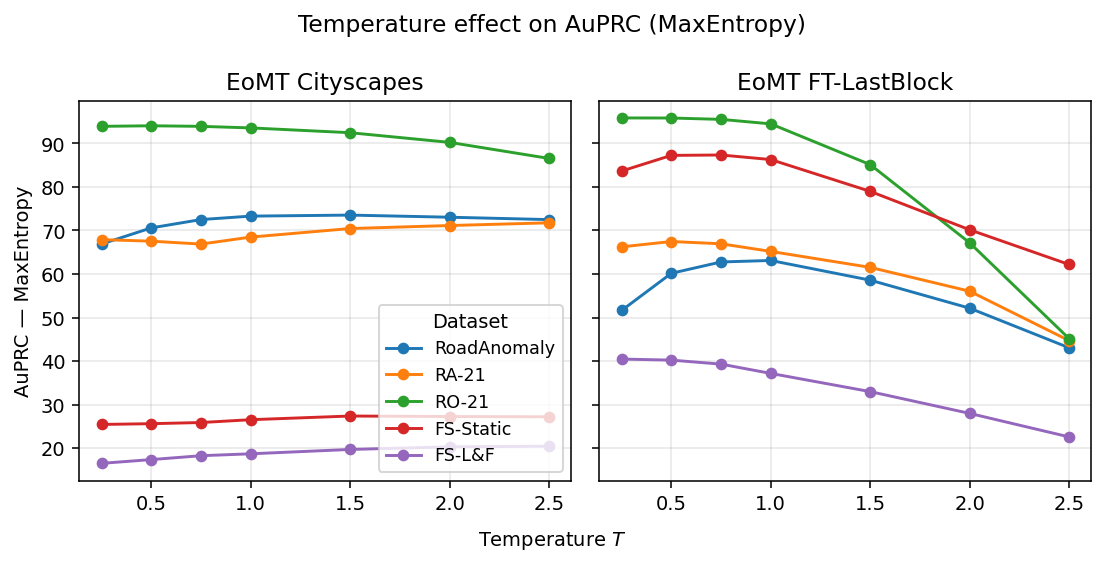
\includegraphics[width=\linewidth]{temp.png}
  \caption{MaxEntropy AuPRC under temperature scaling.}
  \label{fig:temperature}
\end{figure}

\cref{tab:temperature_results,fig:temperature} quantify the absence of a universal temperature. FT-LastBlock selects $T=0.5$ on RA-21, $T=0.25$ on RO-21 and Lost \& Found, $T=0.75$ on FS Static, and $T=1$ on Road Anomaly. Across the broader sweep, RbA is more temperature-sensitive than MaxEntropy and can collapse under flattening.

Selecting temperature by AuPRC does not necessarily improve FPR95. FT-Head RA-21 improves from 73.4 to 80.1 AuPRC at $T=0.25$, but its FPR95 rises from 27.7 to 99.2. Similarly, FT-LastBlock Lost \& Found improves from 37.2 to 40.5 AuPRC while FPR95 worsens from 17.4 to 50.5. Per-dataset best temperatures are therefore oracle analyses rather than deployable calibration choices.

\section{Discussion}
% grammar fix: Comparison of two model
\subsection{Comparison of the Two Models}
For step4, the results are consistent with the training setup of the two models. The Cityscapes checkpoint was trained directly for semantic segmentation on road scenes, so it matches the validation set very well. This explains why it reaches an mIoU of 0.8582.

The COCO checkpoint was trained for panoptic segmentation on COCO. COCO contains many different object categories, but it is not focused on driving scenes in the same way as Cityscapes. In addition, panoptic segmentation is not exactly the same as semantic segmentation. For this reason, the COCO panoptic output has to be converted into semantic labels before computing mIoU.

The qualitative images show the same trend. The Cityscapes model produces outputs that are closer to the ground truth semantic masks. The COCO model produces panoptic-style regions with object boundaries.

The main limitation of this evaluation is the class mapping. A common label space is used to make the comparison possible, but the mapping between COCO and Cityscapes is still not perfect. Some Cityscapes classes are missing or defined differently in COCO.

\subsection{Fine-tuning}
\begin{figure*}[t]
    \centering
    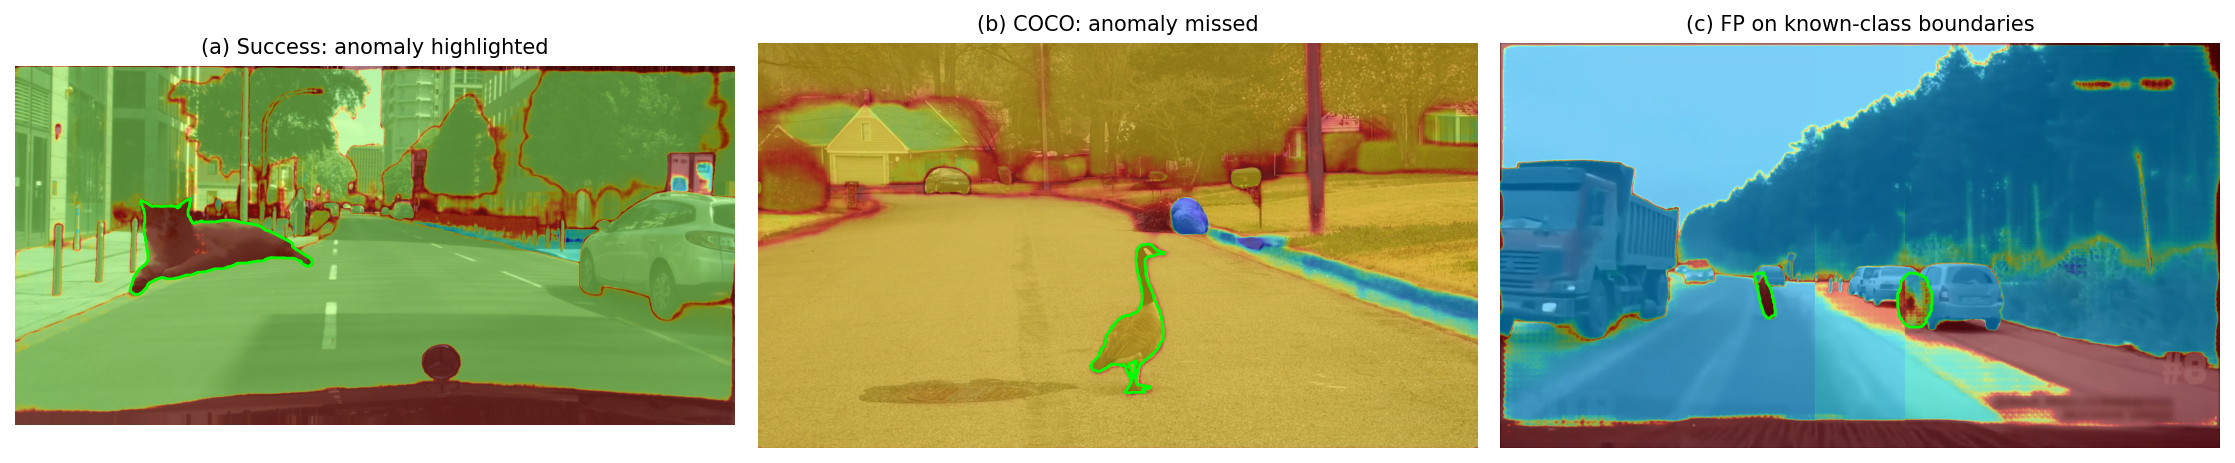
\includegraphics[width=\textwidth]{qualitative.png}
    \caption{Qualitative anomaly-segmentation examples. Green contours denote ground truth, while heatmaps show per-image normalized anomaly scores for visualization only. The examples highlight successful localization and two complementary failure modes: confident anomaly acceptance and uncertainty on known-class boundaries.}
    \label{fig:qualitative}
\end{figure*}

For step 5 in the light of observed results our interpretation is that COCO baseline is low because COCO and Cityscapes have different structure such as label spaces and domains. The head-only fine-tuning approach substantially improved mIoU because EoMT already has great visual capabilities. It scores below the target model mainly it is not really trained first for Cityscapes. As our last experiment in this Last-block fine-tuning is giving us good signals, but it is not very dramatic compared to head-only tuning. 

This can be caused by the resolution of images, limited epochs due to the need for more compute power, and COCO Cityscapes differences. Since our experimentation plays a role in exploring how close we can get by basic and cheap methods, further trials might have more promising results.

\subsection{Pixel-based baselines}
% \begin{figure*}[t]
%     \centering
%     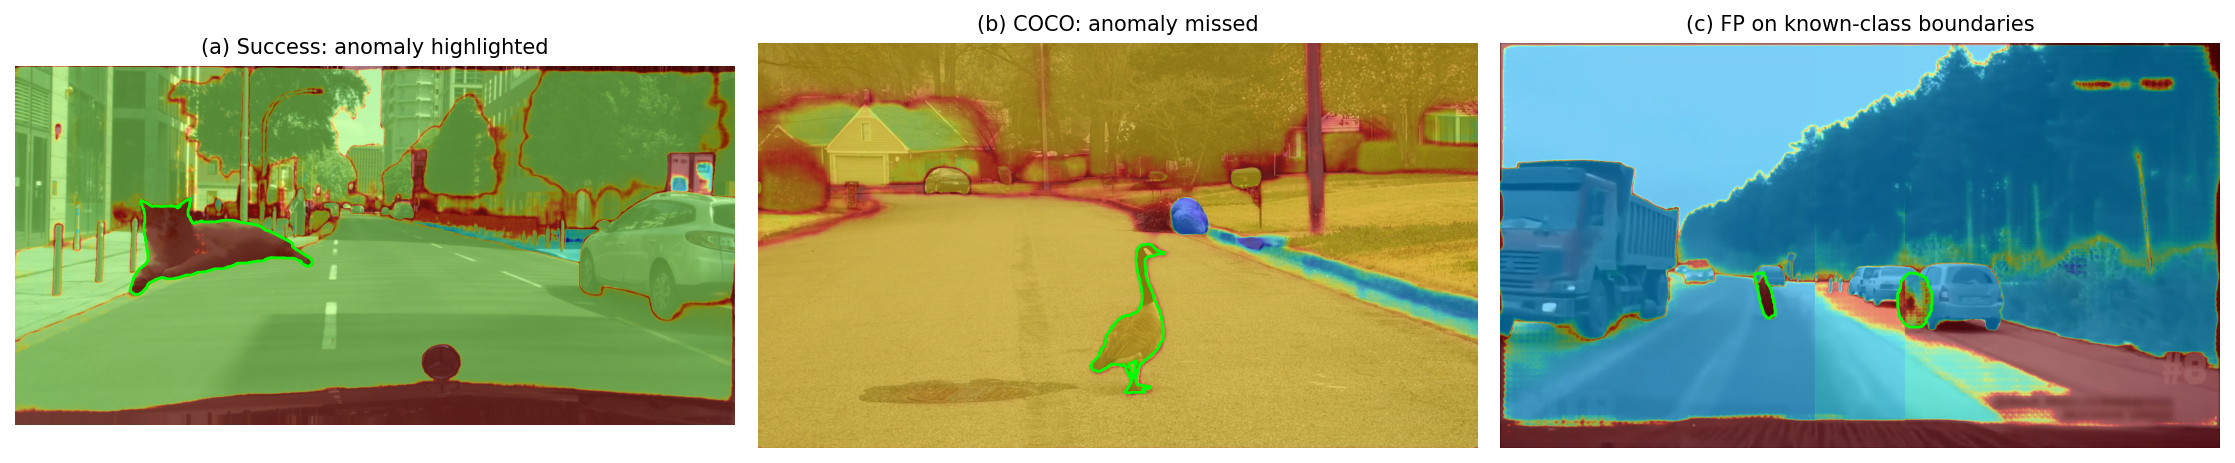
\includegraphics[width=\textwidth]{qualitative.png}
%     \caption{Qualitative anomaly-segmentation examples. Green contours denote ground truth, while heatmaps show per-image normalized anomaly scores for visualization only. The examples highlight successful localization and two complementary failure modes: confident anomaly acceptance and uncertainty on known-class boundaries.}
%     \label{fig:qualitative}
% \end{figure*}

For what concerns pixel-based baselines, the MaxLogit method consistently showed the best performances, as shown by table~\ref{tab:pixel-based baselines}, owing that to the preservation of the magnitude of the scores and to the absence of the exponentiality present in the Softmax, which leads to skewed confidence, and which is also the reason for the closeness of results between MaxEntropy and Maximum Softmax Probability.

The difference in scores observed across datasets stems from the disparity in anomaly size and label imbalance, and averaging the results across the datasets holds little value, with in-dataset performance being much more expressive.

\subsection{Mask-based baselines}
COCO's 133-class vocabulary includes many objects treated as anomalies by road-scene benchmarks, so the raw checkpoint can confidently accept them instead of rejecting them (Fig.~\ref{fig:qualitative}b). Replacing its head with 19 Cityscapes classes yields a large improvement. However, deeper fine-tuning is not uniformly better: FT-LastBlock improves average AuPRC and four-of-five MaxEntropy FPR95 values relative to FT-Head, but fails sharply on RA-21. The best checkpoint therefore depends on anomaly type.

MSP, MaxLogit, and MaxEntropy share the aggregated EoMT semantic score and consequently produce similar rankings; MaxEntropy is the most consistent. RbA is effective when anomalies are rejected by all known classes, but fails when a known class confidently claims them(Fig.~\ref{fig:qualitative}c). Temperature scaling is similarly dataset- and metric-dependent.

\section{Conclusion}

In this project, we carried out a series of experiments on road-scene understanding and anomaly detection using both pixel-based and mask-based segmentation models. We first used ERFNet as a traditional baseline, and then compared different EoMT checkpoints on Cityscapes. The results showed that the original COCO-trained EoMT suffers from domain and label-space mismatch when evaluated on Cityscapes. After fine-tuning, both the head-only and last-block versions improved the semantic segmentation performance, showing that adapting the model to the target dataset is important. For anomaly detection, the experiments also showed that mask-based models combined with post-hoc scores such as MaxEntropy can be useful for detecting out-of-distribution objects in road scenes. Finally, temperature scaling can help in some cases, but its effect depends strongly on the dataset and therefore needs to be tuned carefully.


\section{Acknowledgments}
\begin{itemize}
    \item Generative AI tools were not used for writing the project report.
    \item Generative AI tools were used to just speed up development of code for the experiments
    \begin{itemize}
        \item Codex 5.5, Claude
        \item OpenAI, Anthropic
        \item They were used to review the scripts we have made and guide us to optimize our codes to not exceed the colab runtime limits.
        Human supervision and engineering judgment are made in the whole process.
        
    \end{itemize}
    \item All group members are responsible for these declarations.
\end{itemize}

\section{Revision Notes}
Following the initial submission, we carefully re-examined the original papers for two key terms used throughout this report. First, EoMT was defined incorrectly in the abstract. Upon reviewing Kerssies et al.~\cite{kerssies2025your}, we confirmed the correct expansion is "Encoder-only Mask Transformer", referring to the architecture's use of a ViT encoder without a separate decoder. Second, the original work by Nayal et al.~\cite{nayal2023rba} defines RbA as "Rejected by All", meaning a pixel is flagged as anomalous when it is rejected by all known classes. Both definitions have been corrected in the abstract accordingly. In addition, we have provided the full definitions of all acronyms at their first occurrence in the text.

{\small
  \bibliographystyle{ieeenat_fullname}
  \bibliography{refs}
}
\end{document}
